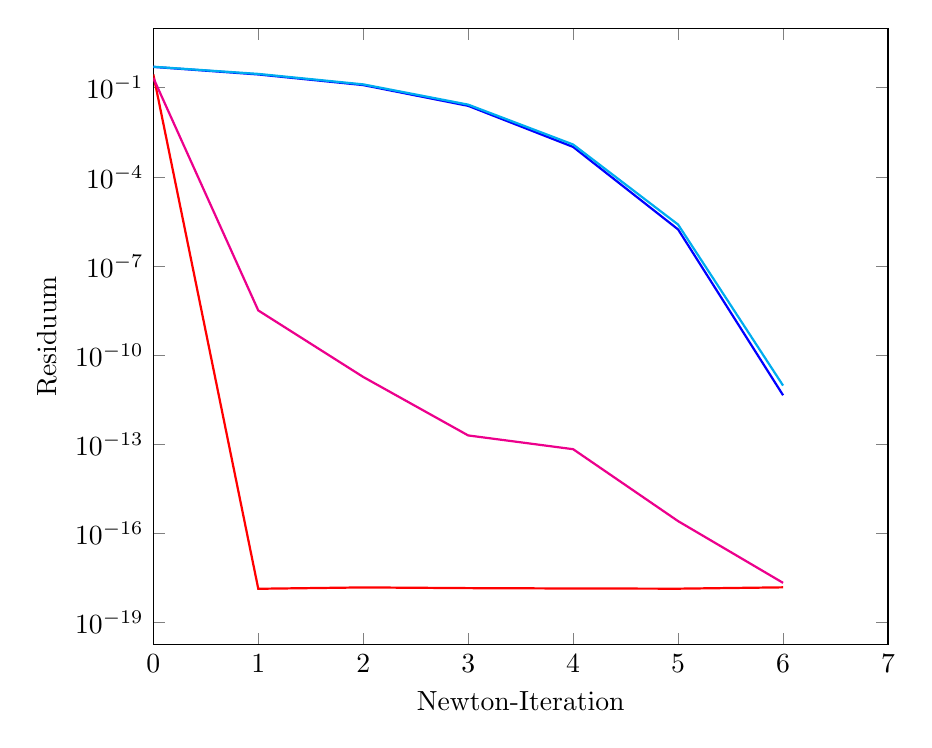
\begin{tikzpicture}[every plot/.append style={thick}] 
\begin{axis}[ 
label style={font=\normalsize}, 
xlabel={Newton-Iteration}, 
ylabel={Residuum}, 
xmin=0, xmax=7, 
ymode=log, 
ymin=0, ymax=10, 
width=0.9\textwidth, 
grid style=dashed, 
] 
\addplot[ 
color=blue, 
] 
coordinates { 
(0, 4.99e-01)(1, 2.78e-01)(2, 1.22e-01)(3, 2.44e-02)(4, 1.01e-03)(5, 1.69e-06)(6, 4.44e-12)}; 
\addplot[ 
color=red, 
] 
coordinates { 
(0, 2.79e-01)(1, 1.36e-18)(2, 1.51e-18)(3, 1.43e-18)(4, 1.39e-18)(5, 1.37e-18)(6, 1.52e-18)}; 
\addplot[ 
color=cyan, 
] 
coordinates { 
(0, 5.06e-01)(1, 2.90e-01)(2, 1.29e-01)(3, 2.68e-02)(4, 1.22e-03)(5, 2.46e-06)(6, 9.40e-12)}; 
\addplot[ 
color=magenta, 
] 
coordinates { 
(0, 2.13e-01)(1, 3.17e-09)(2, 1.83e-11)(3, 1.97e-13)(4, 6.78e-14)(5, 2.57e-16)(6, 2.15e-18)}; 
\end{axis} 
\end{tikzpicture} 
